\section{Force Distribution in a Spherical Joint Model}

\subsection{Problem Statement}
A biomechanics team models a spherical joint system with radius \textbf{7.5 units}, where the \textbf{joint force density} at a point $(x, y, z)$ is described by:
$$I(x,y,z) = 600.17x^{2} + 600.17y^{2} + 600.17z^{2}$$
Compute the total joint force in the system using \textbf{spherical coordinates}.

\subsection{Detailed Solution}
\textit{ Sol. }
\begin{equation*}
	\begin{aligned}
		              & \begin{cases}
			                I(\rho, \theta, \phi) & = 600.17(x^{2} + y^{2} + z^{2} ) = 600.17\rho^2 \\
			                dV                    & = \rho^2 \sin\phi \, d\rho \, d\phi \, d\theta
		                \end{cases}                                                                       \\[1em]
		\Rightarrow F & = \int_{0}^{2\pi} \int_{0}^{\pi} \int_{0}^{7.5} (600.17\rho^2)(\rho^2 \sin\phi) \, d\rho \, d\phi \, d\theta                                  \\
		              & = 600.17 \left( \int_{0}^{7.5} \rho^4 \, d\rho \right) \left( \int_{0}^{\pi} \sin\phi \, d\phi \right) \left( \int_{0}^{2\pi} d\theta \right) \\
		              & = 600.17 \Big[ \frac{\rho^5}{5} \Big]_{0}^{7.5} \Big[ -\cos\phi \Big]_{0}^{\pi} \Big[ \theta \Big]_{0}^{2\pi}                                 \\
		              & = 600.17 \left( \frac{151875}{32} \right) \left( 2 \right) \left( 2\pi \right)                                                                \\
		              & \approx \boxed{35,794,842.8185}
	\end{aligned}
	\label{eq:stu4q2}
\end{equation*}

\subsection{Matlab Implementation}
\begin{figure}[H]
	\begin{center}
		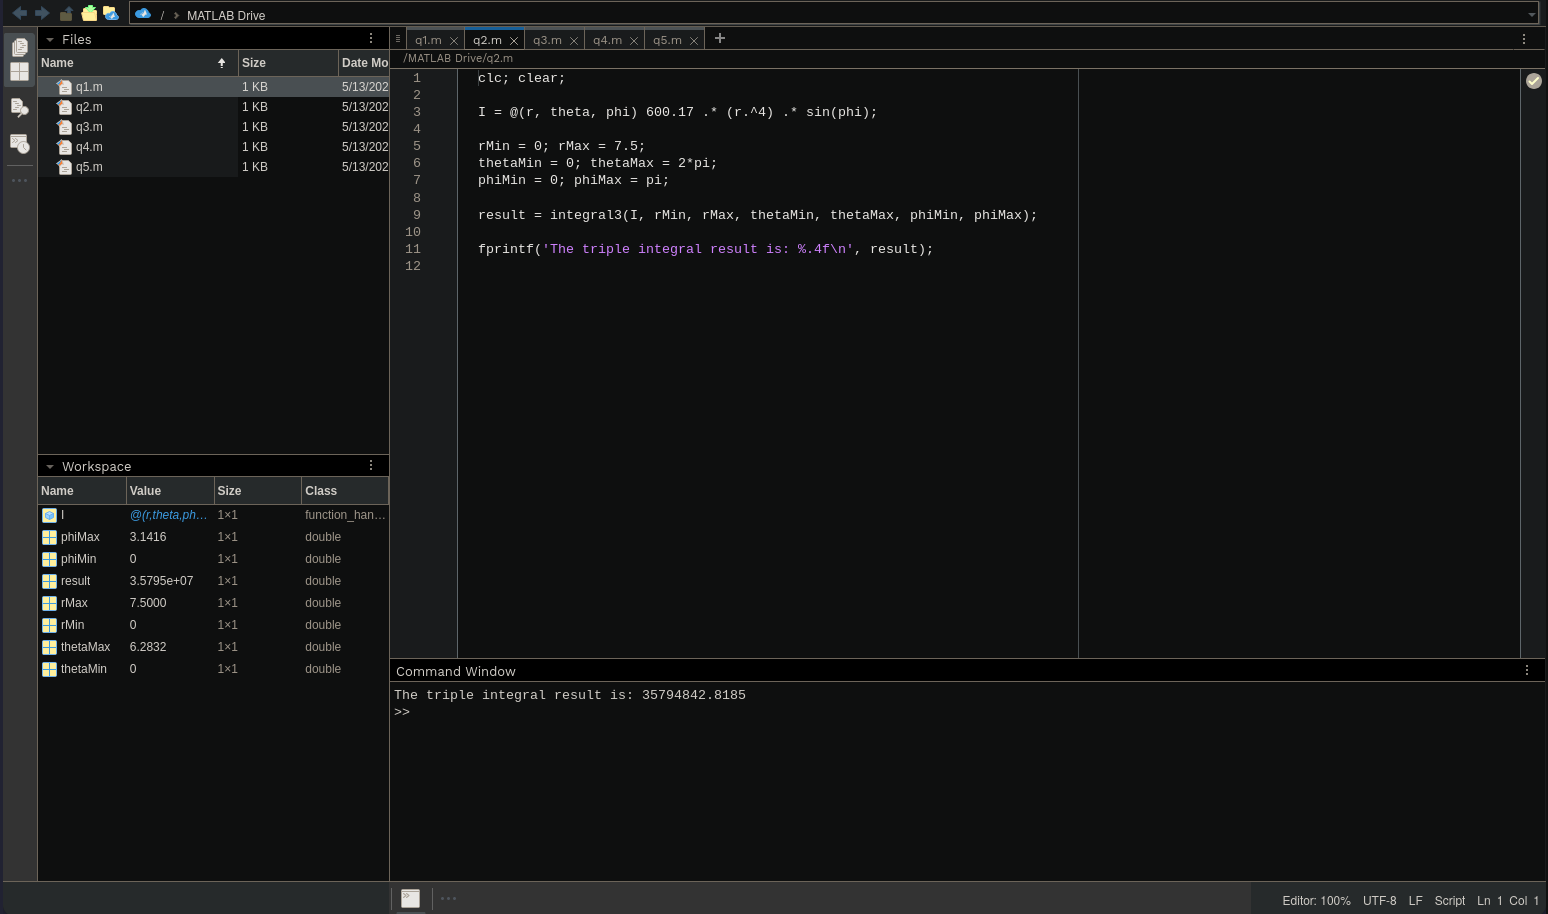
\includegraphics[width=0.95\textwidth]{figures/stu4q2.png}
	\end{center}
	\caption{Student 04 - Matlab Screenshot}
	\label{fig:stu4q2}
\end{figure}

\subsection{Conclusion}
By converting to spherical coordinates, the total joint force (Equation \ref{eq:stu4q2}) \textbf{does} match the MATLAB output (Figure \ref{fig:stu4q2}).
